\documentclass[%
 reprint,
 amsmath,amssymb,
 aps,
]{revtex4-2}
\usepackage{balance}
\usepackage[%
    margin=10mm,% ако не си принтира 10мм не изглежда грозно, а може да събереш повече текст
    % showframe=true,%
    ]{geometry}
\usepackage[T1,T2A]{fontenc}
\usepackage[utf8]{inputenc}
\usepackage[main=bulgarian, english]{babel}
\usepackage{float}
\AtBeginDocument{\selectlanguage{bulgarian}}
\newcommand{\degree}{^{\circ}}
\usepackage{amsmath}
\usepackage{graphics}
\usepackage{graphicx}
\graphicspath{{.}}
\newcommand{\abs}[1]{\lvert#1\rvert}
\let\phi\varphi
\usepackage{booktabs} % от тук се използва само \midrule може и без него 
\usepackage{dcolumn}
\newcolumntype{d}[1]{D{.}{.}{#1}}
\usepackage[unicode=true,pdfusetitle]{hyperref}
\usepackage[]{siunitx}

% \usepackage[compact]{titlesec}

\begin{document}
% \setlength{\abovedisplayskip}{3pt}
% \setlength{\belowdisplayskip}{3pt}    

\title{Измерване на коефициентът на топлинно разширение на етилов спирт}
\author{Васил Николов}
\date{09.06.2022}
\maketitle
%%\balance
\section{Експериментална установка}

Установката се състои от голяма и малка колба, капилярка с диаметър $d = (1.5 \pm 0.08) \si{mm}$ и термометър. Голямата колба е пълна с вода, и лужи за водна баня на малката колба, в която е сложен спирт. Така се гарантира еднаква температура на спирта в целия обем на малката колба. Когато спиртът се нагрява обемът му се увеличава. Тъй като той се разширява повече от малката колба, спиртът влиза в капилярката, където можем да измерим височината му като функция на температурата.

\section{Теоретична обосновка}

При увеличаване на температурата на спирт неговият обем се променя приблизително линейно, по закона 

\begin{equation*}
    V(T) = V_0 (1 + \lambda (T - T_0))
\end{equation*}

Тук $V_0$ e обемът на спирта при дадена температура, $T_0$, а $\lambda$ е константа, коефициентът на обемно топлинно разширение на спиртът. Ако за дадена температура $T$ обемът на спирта е $V(T)$, и той се е изкачил на разстояние $H$ в капилярката, то 

\begin{gather*}
    V(T) = V_0 + H*\pi R^2 \\
    V(T) = V_0 + V_0 \lambda (T - T_0) \\
    V_k(T) = V_0 + \lambda_0 (T - T_0) \\
    \pi R^2 H = V(T) - V_k(T) \\ 
    H = \frac{V_0 \lambda - \lambda_0}{\pi R^2} (T - T_0)
\end{gather*}

Ако направим графика на $y = H, \ x = T$, очакваме да е права линия с наклон. Така можем да изразим 

\begin{gather*}
    \frac{dy}{dx} = \frac{V_0 \lambda - \lambda_0}{\pi R^2} \\
    \lambda = \frac{\pi R^2 \frac{dy}{dx} + \lambda_0}{V_0} \label{eq:1} \tag{1}
\end{gather*}

По уравнение \eqref{eq:1} можем да пресметнем коефициентът на обемно топлинно разширение на спирта.

\section{Експериментални данни и резултати}

\begin{figure}[H]
    \centering
    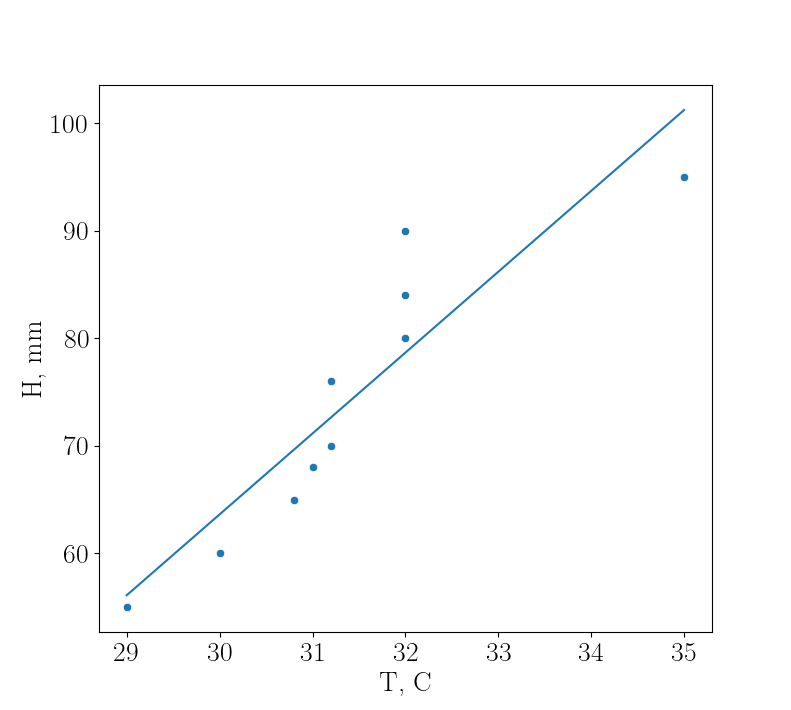
\includegraphics[width=0.9\columnwidth, keepaspectratio=true]{Figure_1.png}
    \caption{Графика на височината на издигане на спирта}
\end{figure}

От графиката определяме, че $\frac{dy}{dx} = (7.5 \pm 1.5) \ \si{mm/K}$. Оказва се, че коефициентът на обемно разширение на стъклото е на порядъци по-малък от този на спирта $(\frac{\Delta V}{V \Delta T}) \approx 2e-6 \ \si{K^{-1}}$, и той няма почти никакво влияние върху крайният резултат. За коефициентът на обемно разширение на спиртът получаваме $\lambda = 1.04e-3 \ \si{K^{-1}} \pm 40\%$, като грешката е дадена за $95\%$ сигурност. Този резултат е в съгласие с табличната стойност $\lambda_t = 1.09e-3 \ \si{K^{-1}}$

\end{document}

